\documentclass{beamer}


\usepackage{amsmath, amsthm, amssymb, bm}
\usepackage{tikz, pgfplots}

\usetikzlibrary{shapes, arrows, positioning, fit, calc}
\pgfplotsset{compat = 1.18}
\usepackage[arrowdel]{physics}

\usepackage{graphicx}
\newcommand\twospace{\,\,}
\newcommand\fourspace{\,\,\,\,}


\graphicspath{ {./images/} }

\usetheme{PaloAlto}
\definecolor{firebrick}{rgb}{0.2, 0.0, 0.53}
\usecolortheme[named = firebrick]{structure}


\setbeamersize{sidebar width left=0cm}

\title{Subgradient Method}
\author[]{Chirag Mehta: ai20btech11006@iith.ac.in}
\institute{Indian Institute Of Technology, Hyderabad}
\date{}
\renewcommand{\vec}[1]{\underline{#1}}

\begin{document}
\begin{frame}{AI2101 - Convex Optimization Project}
\titlepage
\end{frame}

\begin{frame}{Introduction}
    Subgradient method is a simple algorithm used to minimize non-differentiable convex functions. This method is similar to vanilla gradient method which is used to optimize differentiable functions.~\cite{boyd2003subgradient}
\end{frame}

\begin{frame}{Algorithm}
    Lets say we have a nondifferentiable function $f\, : \, \mathbb{R}^n\to \mathbb{R}$. The update rule of subgradient method says
    \begin{align}
        \vec{x}^{(k+1)} = \vec{x}^{(k)} - \alpha_k\vec{g}^{(k)} \label{eq:subgrad_iter}
    \end{align}
    where $\vec{x}^{(k)}$ is the $k^{th}$ iterate, $\alpha_k$ is the step step size at $k^{th}$ iteration and $\vec{g}^{(k)}$ is any subgradient of $f$ at $\vec{x}^{(k)}$. The subgradient $\vec{g}^{(k)}$ is any vector which satisfies
    \begin{align}
        f(\vec{y}) \geq f(\vec{x}) + \vec{g}^T(\vec{y}-\vec{x})\label{eq:subgrad_condition}
    \end{align}
\end{frame}
\begin{frame}{Subdifferential}
    At a given pozint there can be more than one subgradients, we call the set of subgradients as subdifferential. This algorithm doesn't ensure that the loss always decreases, the loss can and often does increase, we store the best point encountered so far for that reason.
\end{frame}
\begin{frame}{Subdifferential Conti.}
        \begin{theorem}
        If the function f is differentiable at $\vec{x}^{(k)}$ then $\vec{g}^{(k)}$ is equal to the gradient of f at $\vec{x}^{(k)}$
    \end{theorem}
    \begin{proof}
        Substitute $\vec{y} = \vec{x}+\lambda\vec{z},\twospace \lambda > 0$ in \eqref{eq:subgrad_condition}
        \begin{align}
            \frac{f(\vec{x}+\lambda\vec{z}) - f(\vec{x})}{\lambda} \geq \vec{g}^T\vec{z}
        \end{align}
        We can use the limit $\lambda \to 0$
        \begin{align}
            \vec{\nabla}f(\vec{x})^T\vec{z} &\geq \vec{g}^T\vec{z}\\
            \vec{z}^T\left(\vec{\nabla}f(\vec{x})-\vec{g}\right) &\geq 0 \fourspace \forall \vec{z}\\
            \therefore \vec{g} & = \vec{\nabla}f(\vec{x})
        \end{align}
    \end{proof}
\end{frame}
\begin{frame}{Step Size Rules}
    We saw the updation rule in \eqref{eq:subgrad_iter}, the term $\alpha_k$ is called step size. There are a few standard step size rules which are similar to what we use in gradient descent. We will discuss a few different selections for step size
\end{frame}
\begin{frame}{Step Size Rules Conti.}
    \begin{enumerate}
        \item Constant Step Size. $\alpha_k = \alpha$, $\alpha>0$
        \item Constant step length, this means that $\norm{\alpha_k*\vec{g}^{(k)}} = \gamma$, where $\gamma$ is a constant fixed ahead of time.
        \item Square summable but not summable. The step satisfies 
        \begin{align}
            \displaystyle\alpha_k\geq 0,\,\, \sum_{k=1}^\infty \alpha_k^2 < \infty,\,\, \sum_{k=1}^\infty \alpha_k \to \infty
        \end{align}
    \end{enumerate}
\end{frame}
\begin{frame}{Step Size Rules Conti.}
    \begin{enumerate}[4]
        \item Nonsummable diminishing. The step sizes satisfy
        \begin{align}
            \displaystyle \alpha_k \geq 0,\,\, \lim_{k \to \infty} \alpha_k = 0,\,\, \sum_{k=1}^\infty \alpha_k \to \infty
        \end{align}
        \item Nonsummable diminishing step lengths. The step sizes are chosen as $\alpha_k = \gamma_k /\norm{\vec{g}^{(k)}}$ where
        \begin{align}
            \displaystyle \gamma_k \geq 0,\,\, \lim_{k \to \infty} \gamma_k = 0,\,\, \sum_{k=1}^\infty \gamma_k \to \infty
        \end{align}
    \end{enumerate}
\end{frame}

\begin{frame}{Convergence}
    We can prove that using subgradient method the results would converge in a certain range in at most certain number of steps. There are few key assumptions here
    \begin{enumerate}
        \item $\norm{\vec{g_k}} \leq G\, \forall k$
        \item $\norm{\vec{x}^{(1)}-\vec{x}^*} \leq R$ where $\vec{x}^*$ is the optimal solution.
    \end{enumerate}
\end{frame}

\begin{frame}{Example}
Consider the following problem

\begin{align}
    min\fourspace max\{f_1,f_2,\dots f_n\},\twospace f_i : \mathbb{R} \to \mathbb{R}
\end{align}
This problem is non differentiable but it can be solved using subgradient method. The first step is to calculate the subgradients are all the points that occur in our iterative algorithm. To obtain the subgradients we can directly use the right hand derivative as the subgradients would lie in the interval of left hand gradient and right hand gradient.
\end{frame}

\begin{frame}{Numerical Example}
Consider the following problem of the type maximum of linear functions
\begin{align}
    min\fourspace max\{f_1,f_2,\dots f_5\}
\end{align}
given
\begin{align}
    &f_1(x) = -5x-25\nonumber\\
    &f_2(x) = -3x-10\nonumber\\
    &f_3(x) = -x+1 \nonumber\\
    &f_4(x) = 2x+4\nonumber\\
    &f_5(x) = 5x+20 \nonumber
\end{align}
\end{frame}

\begin{frame}{}
    We will use the subgradient method algorithm to arrive at the optimal solution. There is still uncertainty as to how to choose the step size $\alpha_k$. We will compare a few different step sizes
\end{frame}
\begin{frame}{Numerical Example Conti}
    \textbf{Constant Step Size}
    \begin{figure}[H]
        \centering
        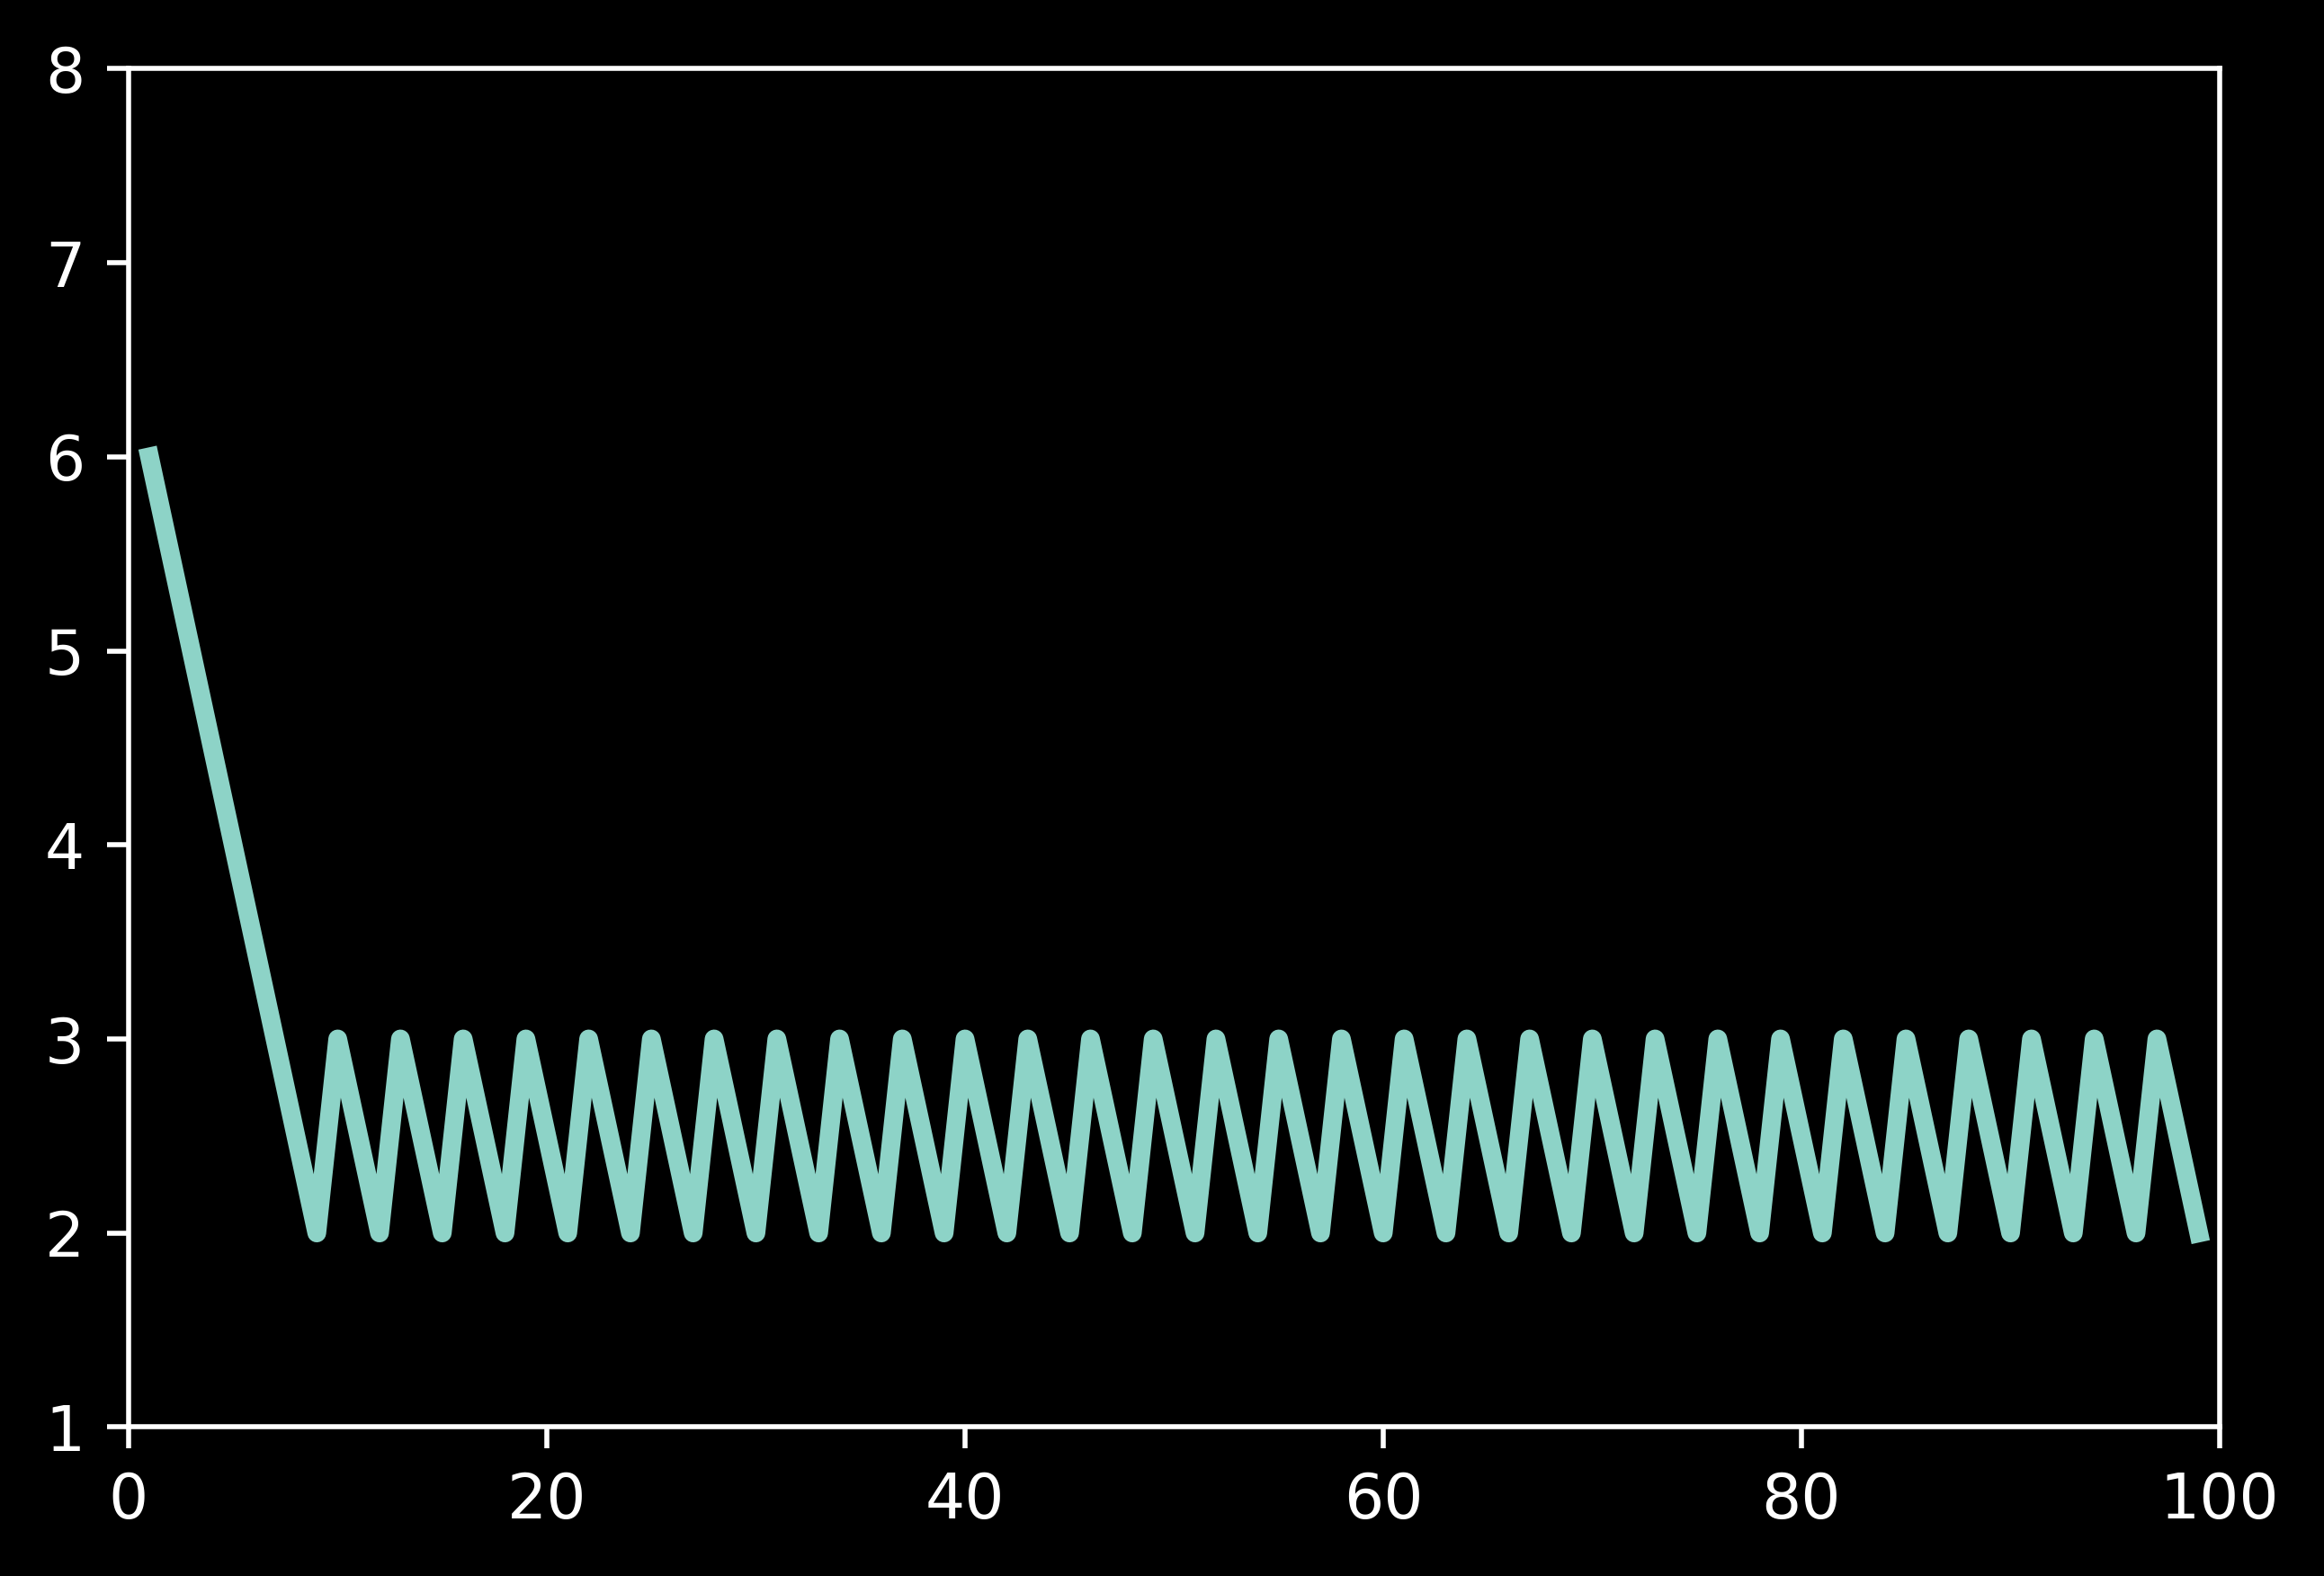
\includegraphics[scale=0.5]{../../step/constantstepsize.png}
        \caption{Constant Step Size}
        \label{constantstepsize}
    \end{figure}
\end{frame}


\begin{frame}{Numerical Example Conti}
    \textbf{Constant Step Length}
    \begin{figure}[H]
        \centering
        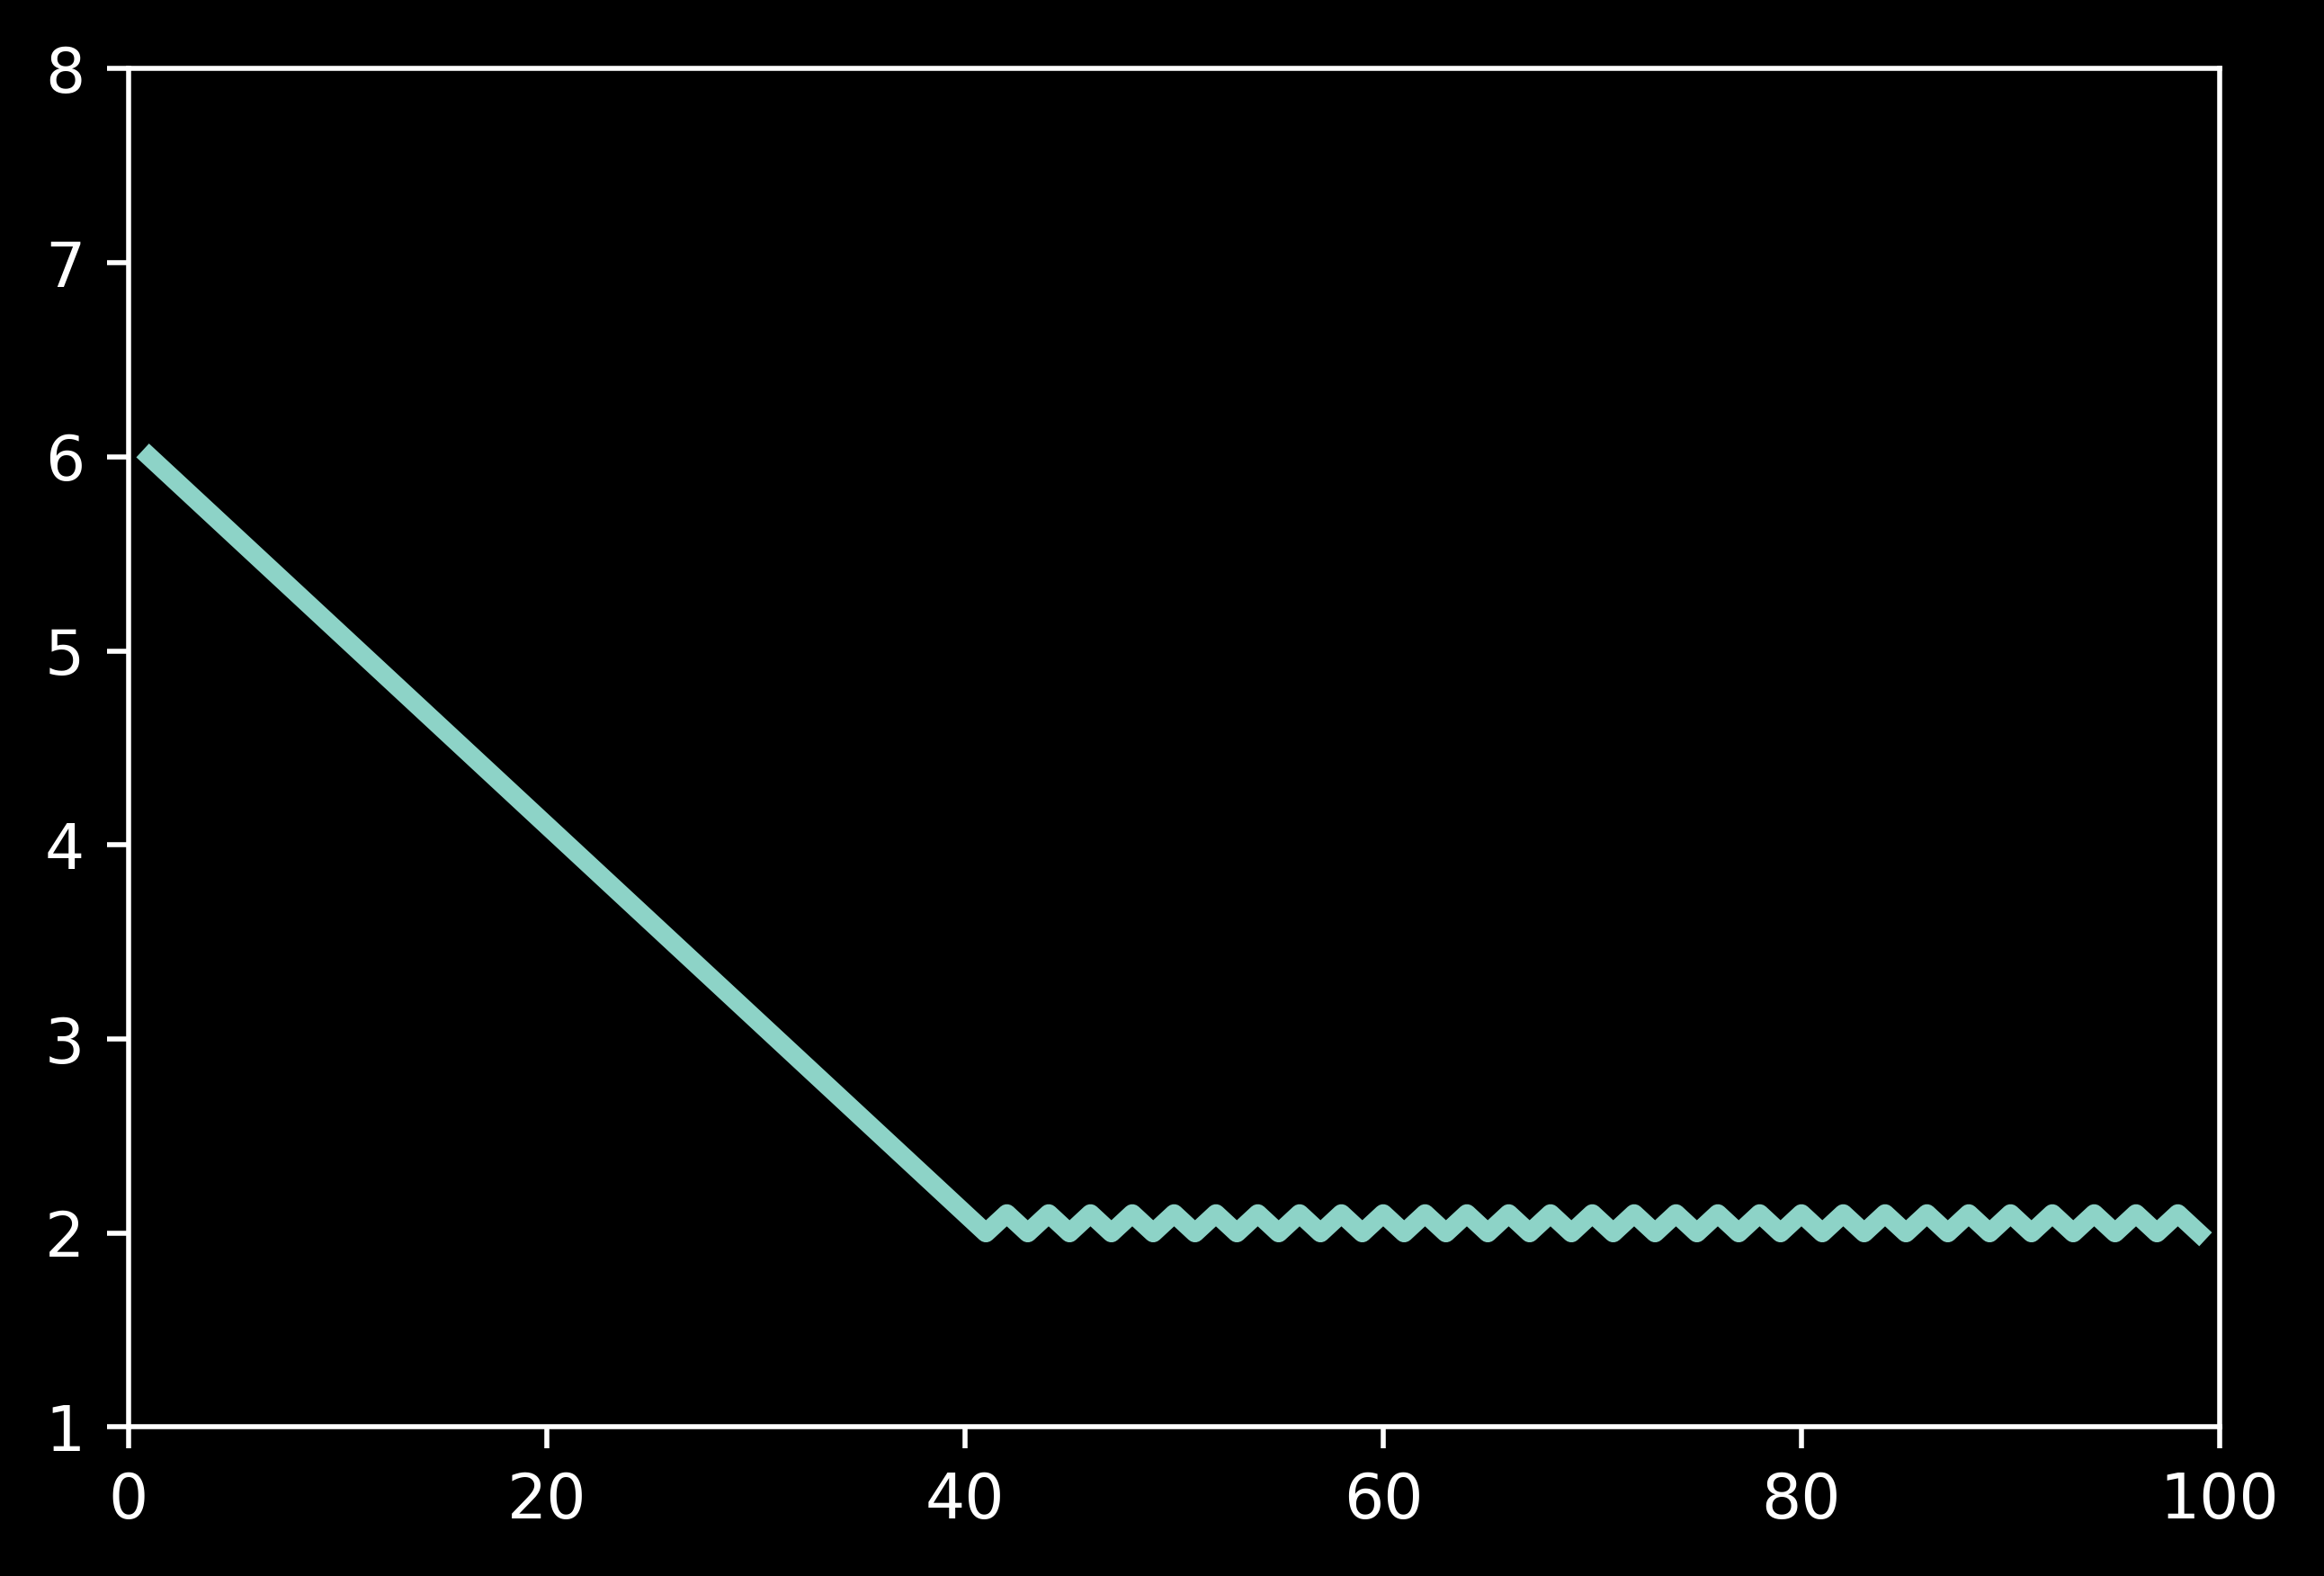
\includegraphics[scale=0.5]{../../step/constantsteplength.png}
        \caption{Constant Step Length}
        \label{constantsteplength}
    \end{figure}
\end{frame}


\begin{frame}{Numerical Example Conti}
    \textbf{Square Summable But Not Summable}
    \begin{figure}[H]
        \centering
        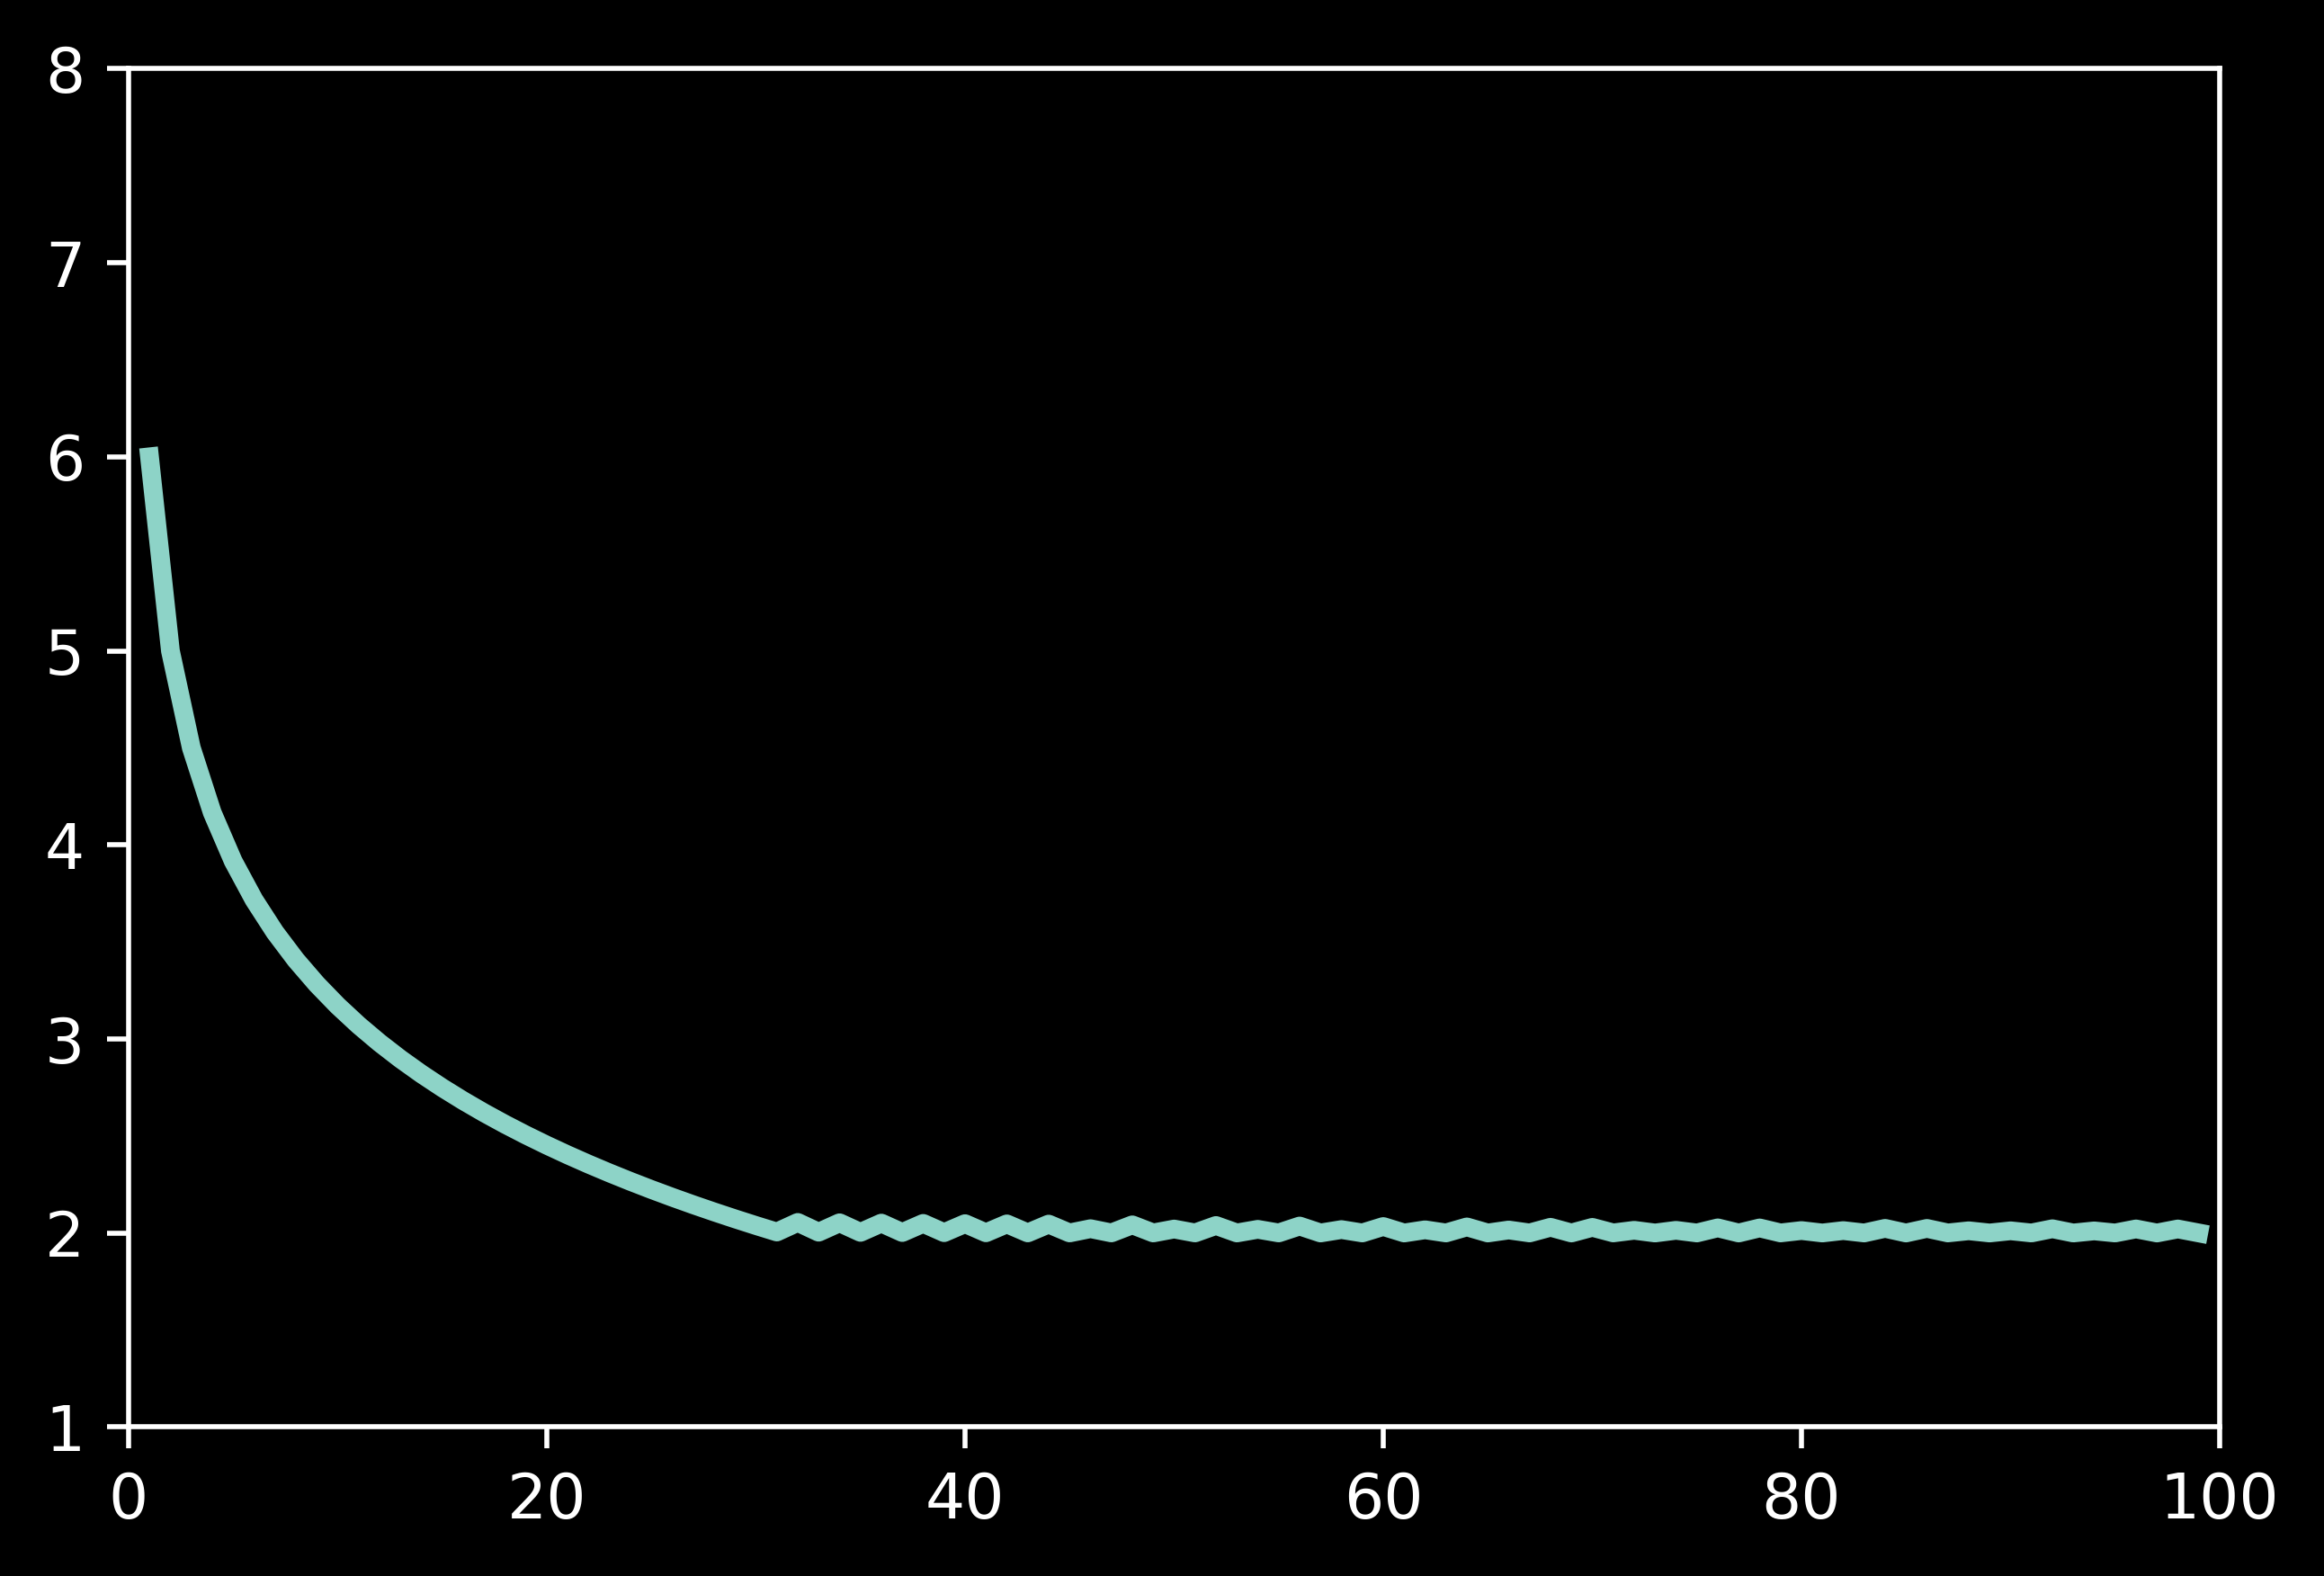
\includegraphics[scale=0.5]{../../step/squaresummablebutnotsummable.png}
        \caption{Square Summable But Not Summable}
        \label{squaresummablebutnotsummable}
    \end{figure}
\end{frame}

\begin{frame}{Numerical Example Conti}
    \textbf{Non Summable Diminishing}
    \begin{figure}[H]
        \centering
        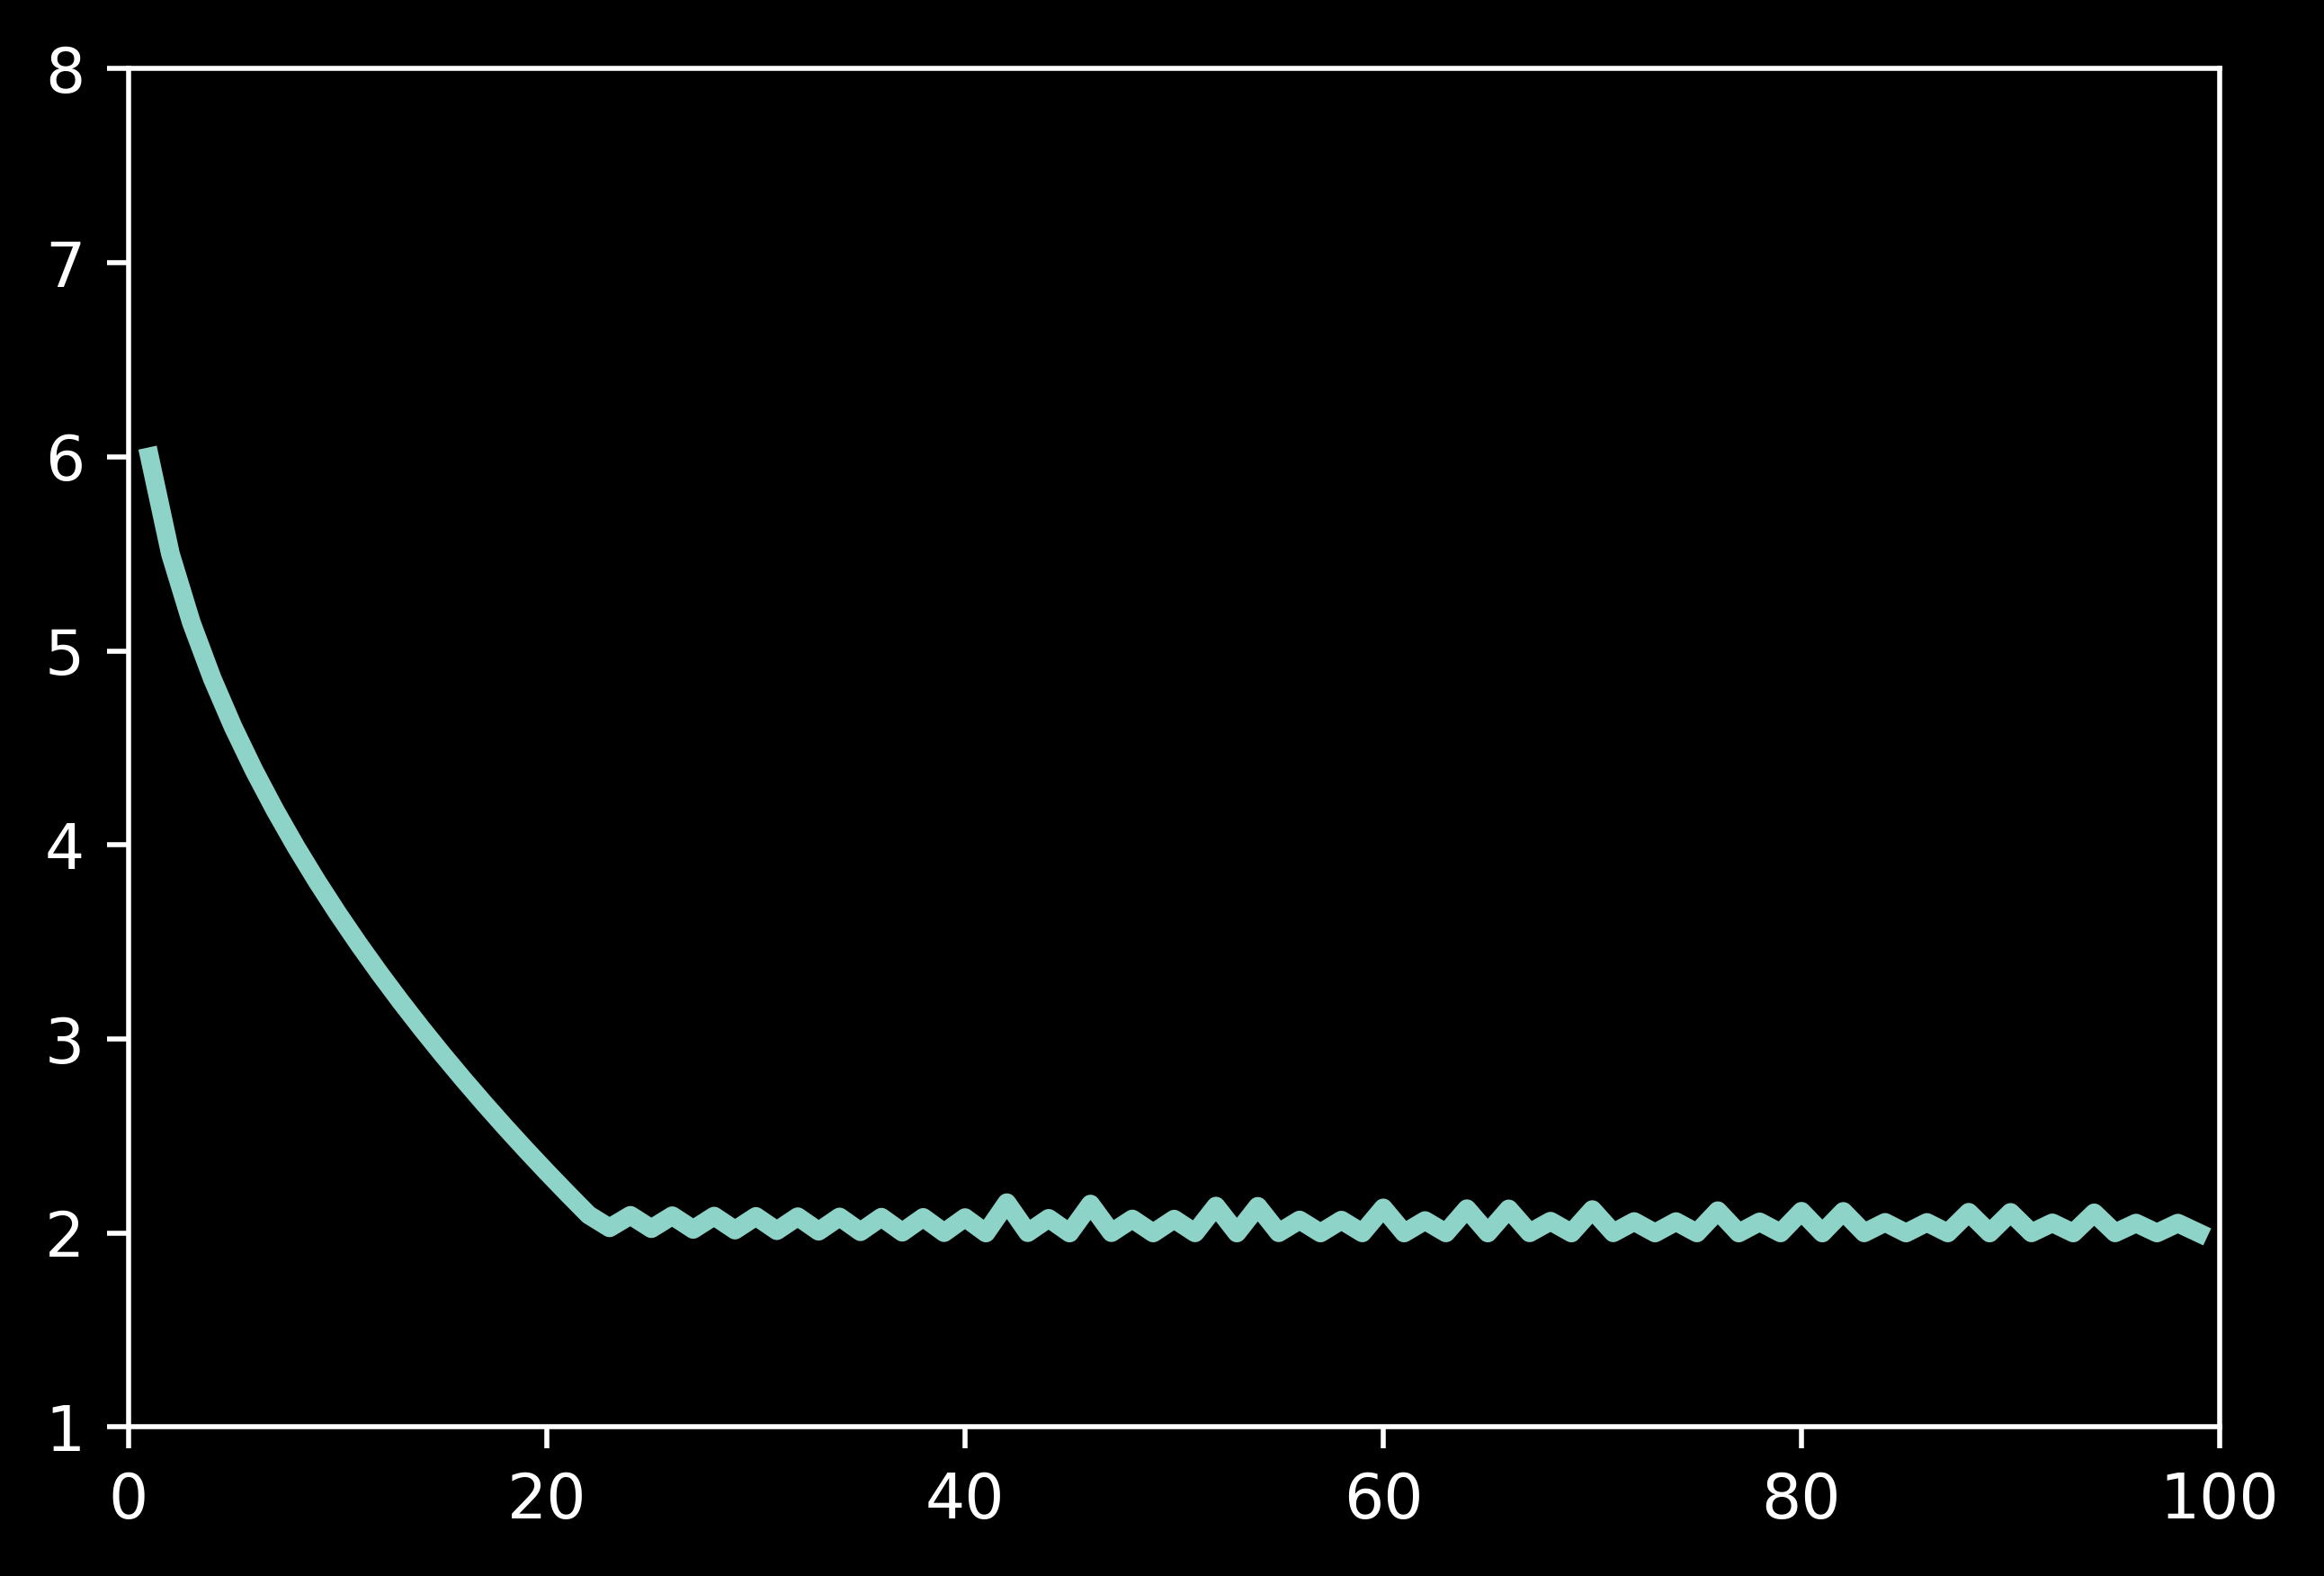
\includegraphics[scale=0.5]{../../step/nonsummablediminishing.png}
        \caption{Non summable diminishing}
        \label{nonsummablediminishing}
    \end{figure}
\end{frame}


\begin{frame}{SVM using subgradient method}
A support vector machine is used for two class classification. The objective is to maximize the slab thickness while still satisfying  few constraints. A hard-margin SVM can be formuated as
\begin{align}
    \begin{split}
        \min_{\vec{w},b}\, &\twospace\vec{w}^T\vec{w}
    \end{split}\\ 
    \text{s.t:}
    \twospace & y_i(\vec{w}^T\vec{x_i}+b)\geq 1
\end{align}
\cite{10.1145/1273496.1273598}We can transform this problem into
\begin{align}
    \min_{\vec{w},b}\, &\twospace\vec{w}^T\vec{w} + \lambda \sum_i \max\left(0, 1-y_i\left(\vec{w}^T\vec{x}+b\right)\right)
\end{align}
\end{frame}

\begin{frame}{SVM using subgradient method Conti.}
    Where $\lambda$ is the trade off factor, the higher is the value of this parameter, the higher is the penalty of voilating the given constraints. This problem is essentially a soft-margin SVM. We can now solve this problem by subgradient method.
\end{frame}

\begin{frame}{SVM using subgradient method Conti.}
    The first step is to calculate the subgradients, 
\begin{align}
    \vec{g}_{\vec{w}} = 2\vec{w}+\frac{1}{n}\times\lambda\displaystyle\sum_i y_i\left(\vec{x_i}\right) \fourspace for\,  y_i\left(\vec{w}^T\vec{x}+b\right) < 1
\end{align}
and
\begin{align}
    g_{b} = \frac{1}{n}\times\lambda\displaystyle\sum_i^{n} y_i \fourspace for\,  y_i\left(\vec{w}^T\vec{x}+b\right) < 1
\end{align}
\cite{boyd2008stochastic}In practice, we tend to use mini-batch subgradient method because of its several advantages such as computational efficiency, stable convergence and faster learning.
\end{frame}

\begin{frame}{SVM results}
    Now, we can use these update rules to train our SVM. Given below are few illustrations of our SVM.

    \textbf{Hard Margin SVM: $\lambda = 1e9$}
    \begin{figure}[H]
        \centering
        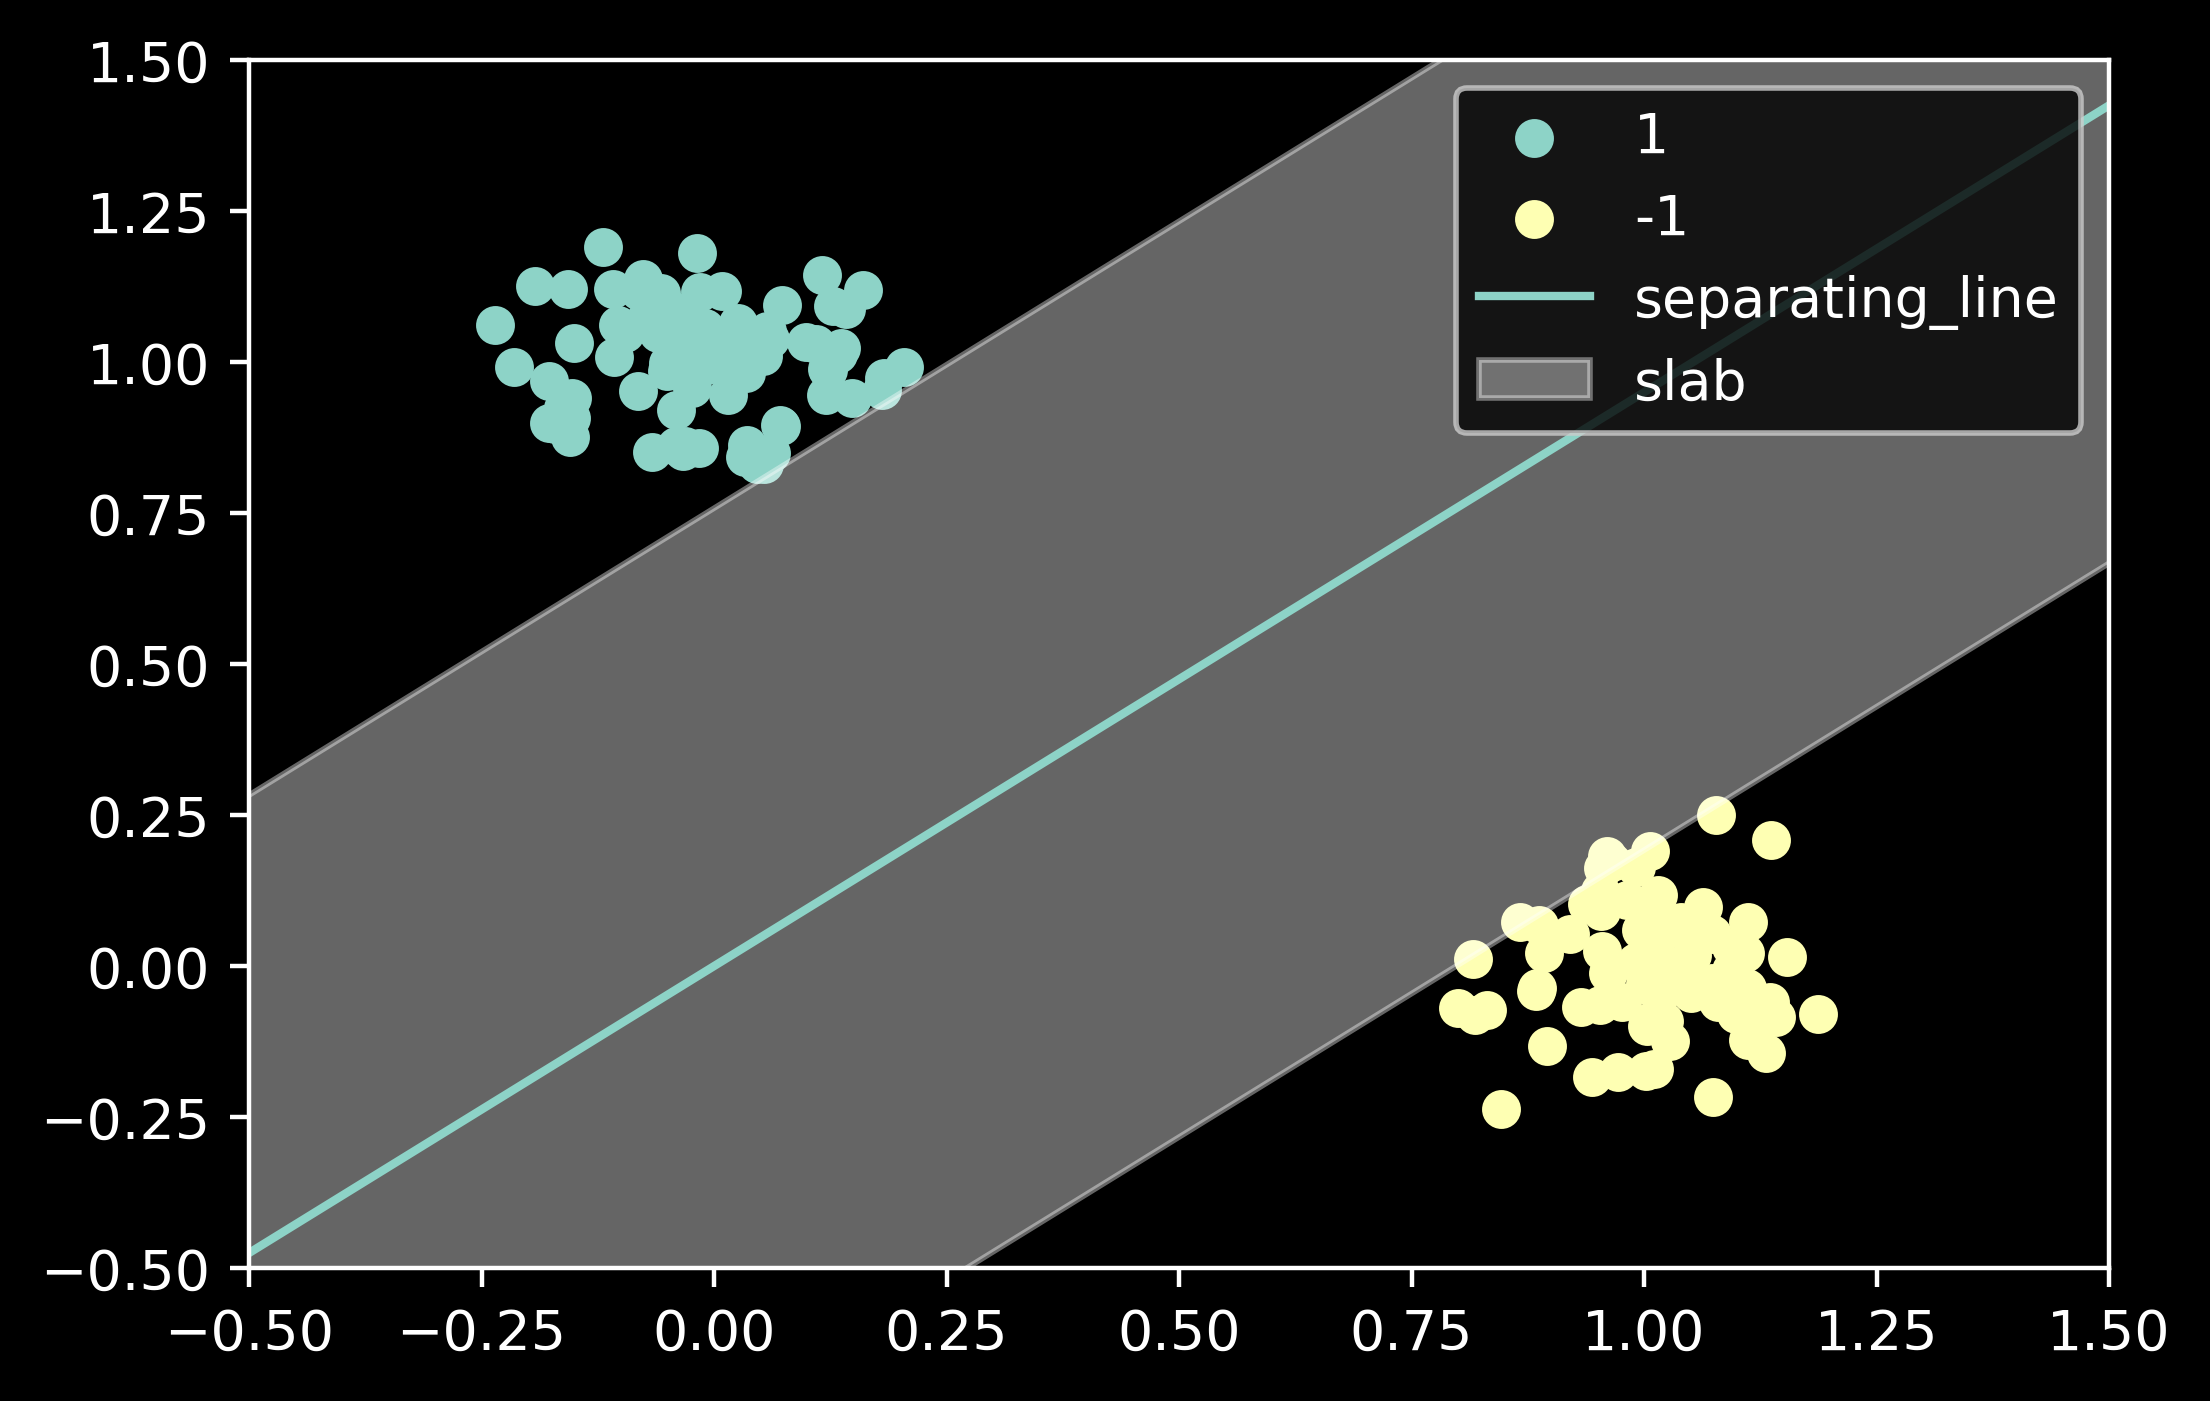
\includegraphics[scale=0.5]{../../results/svm(train_data).png}
        \caption{Hard Margin SVM}
        \label{hardmargin}
    \end{figure}
\end{frame}

\begin{frame}{SVM results}
    \textbf{Soft Margin SVM: $\lambda = 100$}
    \begin{figure}[H]
        \centering
        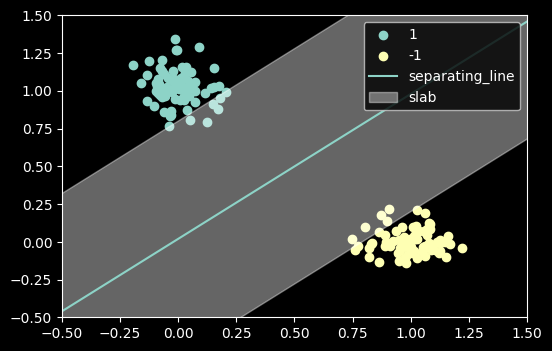
\includegraphics[scale=0.5]{../../results/softmargin.png}
        \caption{Soft Margin SVM}
        \label{softmargin}
    \end{figure}
\end{frame}

\begin{frame}{Spam Classification using SVM}
    Spam classification problem can be solved by soft margin SVM using linear kernel. The text in email can be tokenized and encoded in higher dimension. For our purposes, \emph{sklearn.feature\_extraction.text.CountVectorizer}~\cite{scikit-learn} can be used. The SVM written from scratch using numpy is able to attain an accuracy of $98.56\%$. The code can be found \href{https://github.com/cmaspi/subgradient\_method/blob/main/code/spam\_classification.ipynb}{here}
\end{frame}    

\begin{frame}{Heavy Ball Method}
    Heavy-ball method which is same as momentum method is used for a faster convergence and reduced oscillations. The update rule can be represented as
    \begin{align}
        \vec{x}^{(k+1)} = \vec{x}^{(k)} - \alpha_k\vec{g}^{(k)} + \beta\left(\vec{x}^{(k)}-\vec{x}^{(k-1)}\right)
    \end{align}
    I've implemented momentum method \href{https://github.com/cmaspi/subgradient_method/blob/main/code/svm_numpy.py}{here}
\end{frame}

{\small
\bibliographystyle{ieee_fullname}
\bibliography{egbib}
}


%-------------------------------------------------------------------%
\end{document}
